\documentclass{beamer}

\usetheme{Madrid}
\usecolortheme{seahorse}
\setbeamertemplate{navigation symbols}{}
\setbeamertemplate{footline}[frame number]

\usepackage[french]{babel}
\usepackage[utf8]{inputenc}
\usepackage[T1]{fontenc}
\usepackage{amsmath,amsfonts,amssymb}
\usepackage{graphicx}
\usepackage{booktabs}
\usepackage{graphicx}
\usepackage{caption}
\usepackage{subcaption}

% ---- Infos présentation ----
\title{Centralized Training -- Decentralized Execution (CTDE)}
\author{Supervisé par : AIT OMAR Driss\\
            Préparé par : AIT AHMED OULHAJE Soulaimane}
\institute{Master AIDC — FST Béni Mellal}

\begin{document}

%------------------------------------------------
\begin{frame}
\titlepage
\end{frame}

%------------------------------------------------
\begin{frame}{Plan de la présentation}
\tableofcontents
\end{frame}

%------------------------------------------------
\section{Single-Agent Reinforcement Learning}

\begin{frame}{Motivation – Pourquoi le Deep RL ?}
\begin{itemize}
    \item Méthodes tabulaires (Q-learning classique) → impossibles sur grands espaces
    \item Approximations linéaires → trop limitées
\end{itemize}

  

Exemples concrets :
\begin{itemize}
    \item Jeux Atari (pixels bruts → état très haut-dimensionnel)
    \item Robotique (capteurs, vision, moteurs continus)
\end{itemize}

 \centering
\textbf{Solution clé :} Réseaux de neurones profonds + RL = \alert{Deep Reinforcement Learning}
\end{frame}

\begin{frame}{Value-Based vs Policy-Based Methods}

\begin{columns}[T]

\begin{column}{0.48\textwidth}
\textbf{Value-Based (ex: DQN)}\\
\small
Apprend la \textbf{valeur} des actions :\\[0.4em]
$ Q(s,a) = \mathbb{E}[\text{récompense future}] $\\[0.6em]

Politique : $\pi(s) = \arg\max_a Q(s,a)$\\[0.8em]

\small
Avantages :
\begin{itemize}
    \item Exploration facile (ε-greedy)
    \item Très bon sur \textbf{actions discrètes}
\end{itemize}

Inconvénients :
\begin{itemize}
    \item Ne marche pas (ou mal) sur actions continues
    \item Surestimation fréquente (max operator)
\end{itemize}

\end{column}

\begin{column}{0.04\textwidth}
    \phantom{x}
\end{column}

\begin{column}{0.48\textwidth}
\textbf{Policy-Based (Policy Gradient)}\\
\small
Apprend \textbf{directement} la politique :\\[0.4em]
$ \pi_\theta(a|s) $\\[0.6em]

Objectif : $\max J(\theta) = \mathbb{E}_{\pi_\theta}[\sum r_t]$\\[0.6em]

MàJ : $\theta \leftarrow \theta + \alpha \nabla_\theta J(\theta)$\\[0.8em]

\small
Avantages :
\begin{itemize}
    \item Fonctionne très bien sur \textbf{actions continues}
    \item Exploration naturelle (politique stochastique)
\end{itemize}

Inconvénients :
\begin{itemize}
    \item Forte variance → apprentissage instable
\end{itemize}

\end{column}

\end{columns}

\end{frame}

\begin{frame}{Actor-Critic : le meilleur des deux mondes}

\begin{figure}
    \centering
    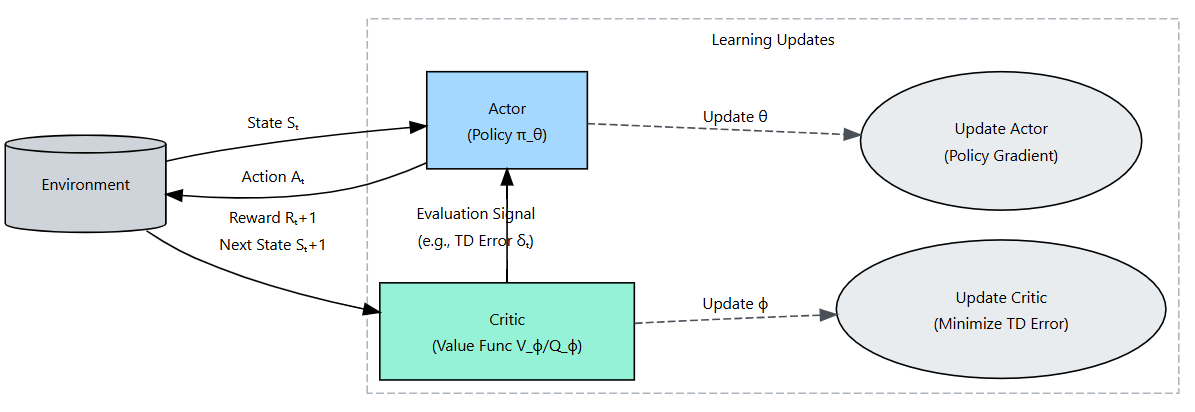
\includegraphics[width=0.75\linewidth]{actor-critic-diagram.png}
\end{figure}

\textbf{Actor} : choisit l'action (Input du réseau cest s)\\
\[ a \sim \pi_\theta(a|s) \]

     
\textbf{Critic} : évalue l'action (Input du réseau cest s ou s et a)\\
\[ V^\pi(s) \quad \text{ou} \quad Q^\pi(s,a) \]

Intuition : 
\begin{itemize}
    \item Actor = conducteur
    \item Critic = instructeur qui donne du feedback
\end{itemize}

\end{frame}


\begin{frame}{Comparaison empirique : DQN vs SARSA vs Actor-Critic}
\centering
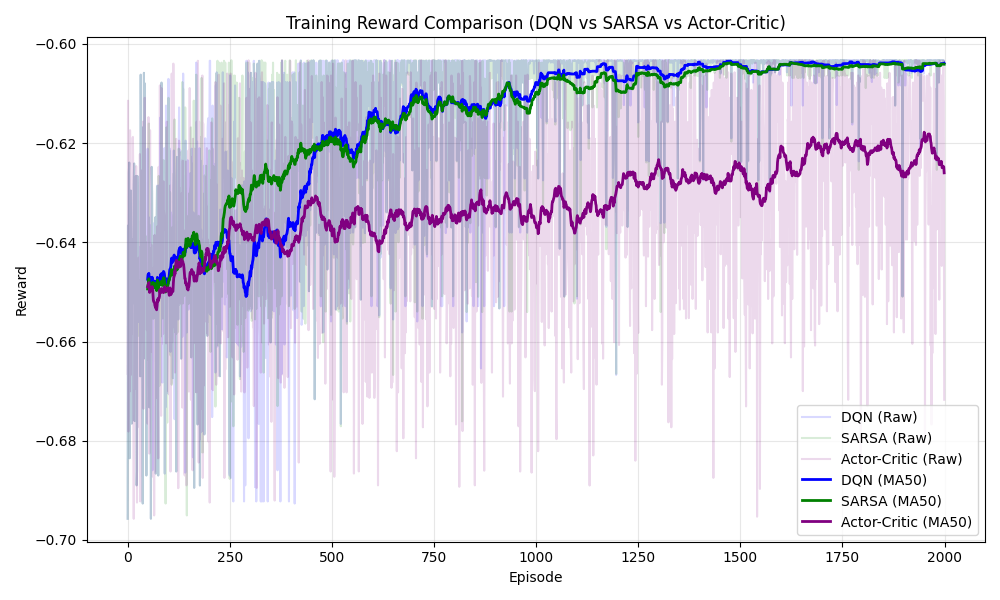
\includegraphics[width=0.72\textwidth]{SingelAgent/comparison/training_reward_comparison.png}

\smallskip

\begin{block}{Performances finales}
\begin{itemize}
    \item \textcolor{blue}{\textbf{DQN}} \quad $\approx -0.605$ \quad (meilleure)
    \item \textcolor{green}{\textbf{SARSA}} \quad $\approx -0.615$
    \item \textcolor{mauve}{\textbf{Actor-Critic}} \quad $\approx -0.620$ à $-0.630$ \quad (la plus faible)
\end{itemize}
\end{block}

\end{frame}

\begin{frame}{Comparaison DQN / SARSA / Actor-Critic – Interprétation}
\frametitle{Interprétation détaillée des comportements}

\begin{columns}[T]
\column{0.48\textwidth}
\textbf{DQN (\textcolor{blue}{bleu})}
\begin{itemize}
    \item Meilleure récompense finale ($\approx -0.605$)
    \item Convergence rapide et stable
    \item Faible variance en phase tardive
    \item Moins de bruit même sur la courbe brute (magenta)
\end{itemize}

\textbf{SARSA (\textcolor{green}{vert})}
\begin{itemize}
    \item Bonne convergence ($\approx -0.615$)
    \item Plus stable que DQN
    \item Mais reste en dessous d’Actor-Critic
\end{itemize}

\column{0.52\textwidth}
\textbf{Actor-Critic (\textcolor{cyan}{cyan})}
\begin{itemize}
    \item Convergence plus lente
    \item Oscillations / forte variance persistante
    \item Performance finale la plus faible
    \item Comportement typique des méthodes value-based avec surestimation
\end{itemize}
\end{columns}

\end{frame}

\begin{frame}{DQN avec un CNN plus lourd – Résultats d'entraînement}
\centering
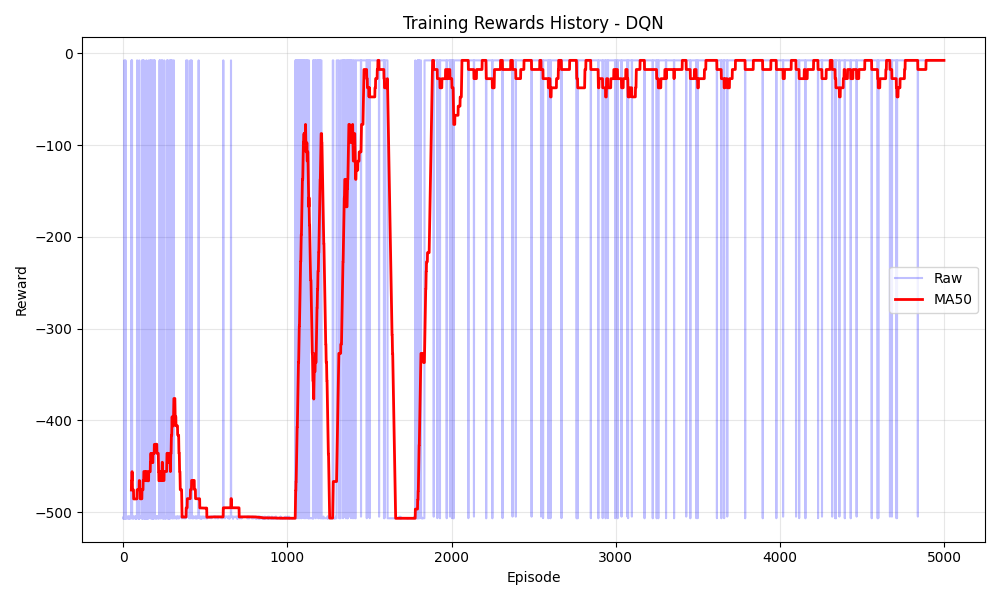
\includegraphics[width=0.70\textwidth]{SingelAgent/resultBigCNN/train/dqn_training_history.png}

\smallskip

\begin{block}{Observations sur la courbe de récompense (DQN + CNN lourd)}
\begin{itemize}
    \item Phase initiale très instable : récompenses extrêmement négatives.
    \item Plusieurs \alert{chutes catastrophiques} visibles
    \item Stabilisation tardive : seulement après ~2000 épisodes la moyenne atteint un plateau autour de −50 / −20
\end{itemize}
\end{block}

\end{frame}

\begin{frame}{Stratégie d'exécution – DQN}
\centering

\includegraphics[width=0.75\textwidth]{SingelAgent/resultBigCNN/train/execution_strategy.png}

\end{frame}

%------------------------------------------------
\section{Multi-Agent Reinforcement Learning}

\begin{frame}{Défis du Multi-Agent RL}
\begin{itemize}
    \item \alert{Non-stationnarité} : les autres agents changent leur comportement
    \item Récompense souvent partagée (coopératif) ou compétitive
    \item Coordination implicite ou explicite ?
    \item Scalabilité (nombre d’agents)
\end{itemize}

  

Trois grandes familles abordées aujourd’hui :
\begin{enumerate}
    \item Apprentissage indépendant (IQL, IDDPG)
    \item CTDE (Centralized Training Decentralized Execution)
    \item Value Decomposition (VDN, QMIX)
    \item MADDPG (Actor-Critic multi-agent)
\end{enumerate}
\end{frame}

\begin{frame}{1. Independent Learners (IQL, IDDPG)}
Chaque agent apprend \alert{tout seul} :
\begin{itemize}
    \item Traite les autres comme partie de l’environnement
    \item Transition vue par l’agent $i$ : $(o_i, a_i, r_i, o_i')$
    \item Ignore totalement les actions/politiques des autres
\end{itemize}

 

Exemples :
\begin{itemize}
    \item \textbf{IQL} : $Q_i(o_i, a_i)$ → comme DQN indépendant
    \item \textbf{IDDPG} : Actor $\mu_i(o_i)$ + Critic $Q_i(o_i, a_i)$
\end{itemize}

  
\alert{Gros problème} : non-stationnarité → oscillations, pas de convergence
\end{frame}

\begin{frame}{Convergence en apprentissage indépendant multi-agent}
\centering

\includegraphics[width=0.75\textwidth]{training_trends.png}

\vspace{0.4em}

\begin{columns}[T]
    \column{0.48\textwidth}
        \textbf{Récompenses (Moving Average)}
        \begin{itemize}
            \item Forte oscillation pendant ~3000 épisodes
            \item Minimum atteint autour de -350 (tous agents)
            \item Amélioration tardive après 3500–4000 épisodes
            \item Convergence lente et instable
        \end{itemize}

    \column{0.52\textwidth}
        \textbf{Taux de succès (\%)}
        \begin{itemize}
            \item Descend jusqu'à ~20–40\% vers le milieu de l'entraînement
            \item Remonte progressivement vers 90–100\% en fin d'entraînement
            \item Tous les agents suivent une trajectoire similaire (mais chaotique)
        \end{itemize}
\end{columns}

\smallskip

\begin{alertblock}{Observation clé}
Oscillations très fortes + lente convergence → signe classique de \alert{non-stationnarité}
\end{alertblock}
\end{frame}

\begin{frame}{Stratégie d'exécution multi-agent – Allocation des couches}
\centering

\includegraphics[width=0.55\textwidth]{MultiAgent/execution_flow.png}

\smallskip

\begin{block}{Interprétation de la stratégie apprise}
\begin{itemize}
    \item Trois agents indépendants décident chacun de l'allocation de leurs couches sur 5 devices
    \item Chaque agent optimise son propre réseau (différentes architectures → complexités différentes)
\end{itemize}
\end{block}

\smallskip\small
$\Rightarrow$ Chaque agent apprend une stratégie \textbf{indépendante}, sans coordination explicite avec les autres
\end{frame}

\begin{frame}{Independent Learners : illustration des problèmes théoriques}

\begin{alertblock}{Lien direct avec la théorie}
\begin{itemize}
    \item \alert{Non-stationnarité} : les autres agents changent leur comportement → l'environnement perçu par chaque agent n'est pas stationnaire
    \item Conséquences observées : oscillations, pas de convergence stable avant très longtemps
    \item Pas de coordination : allocation fragmentée et non optimale globalement
\end{itemize}
\end{alertblock}

\smallskip\centering
$\Rightarrow$ Ces résultats confirment pourquoi l'apprentissage indépendant est limité en multi-agent coopératif
\end{frame}

\begin{frame}{2. CTDE – Centralized Training Decentralized Execution}
\centering
\Large\textbf{La norme actuelle en MARL coopératif}

 \vspace{0.8em}

\begin{columns}[T]
\column{0.52\textwidth}
    \textbf{Training (centralisé)} \\
    Critic voit \alert{tout} : observations + actions globales \\
    → Environnement stationnaire pendant l’apprentissage

\column{0.48\textwidth}
    \textbf{Exécution (décentralisée)} \\
    Chaque agent utilise seulement $o_i$ \\
    \[ a_i = \pi_i(o_i) \]
    → Pas de communication à l’inférence
\end{columns}

 \vspace{0.7em}

\textbf{Avantage clé} : coordination apprise sans dépendance runtime
\end{frame}

\begin{frame}{3. Value Decomposition – VDN}
Objectif : factoriser la valeur jointe $Q_{tot}$ à partir des $Q_i$ individuels. Au lieu que chaque agent apprenne séparément, On apprend une valeur d’équipe, la valeur d'equipe cest somme des valeurs individuelles dans 

  
\begin{center}
    \textbf{VDN (Value Decomposition Networks)}
\end{center}
\[ Q_{tot}(\mathbf{o},\mathbf{a}) = \sum_{i=1}^N Q_i(o_i, a_i) \]

Avantages :
\begin{itemize}
    \item met à jour tous les agents en même temps.
    \item Coordination implicite
    \item Très simple
\end{itemize}

Inconvénients :
\begin{itemize}
    \item \alert{Pas de coordination non-linéaire}
    \item Hypothèse d’additivité trop forte
\end{itemize}
\end{frame}

\begin{frame}{Récompenses individuelles pendant l'entraînement}
\centering

\includegraphics[width=0.65\textwidth]{MultiAgentVDN/training_agent_rewards.png}


\begin{block}{Observations clés sur les récompenses par agent}
\begin{itemize}
    \item Trois agents indépendants avec récompenses très corrélées au début
    \item Forte variance et oscillations pendant les 2000–2500 premiers épisodes
    \item Minimum atteint autour de -400 / -450 (tous agents)
    \item Amélioration progressive après ~2000 épisodes → plateau autour de -50 / 0 vers la fin
\end{itemize}
\end{block}

\smallskip\small
$\Rightarrow$ Les agents évoluent de manière relativement synchronisée, mais avec beaucoup d'instabilité initiale
\end{frame}

\begin{frame}{Retour d'équipe global et synthèse des tendances}
\centering
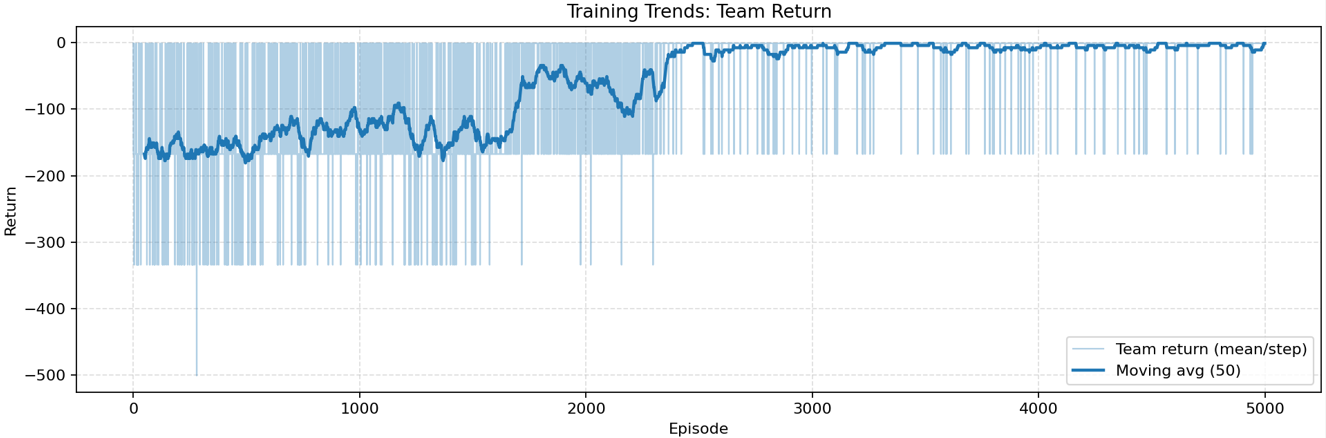
\includegraphics[width=0.75\textwidth]{VDNHist.png}

\vspace{0.4em}

\begin{block}{Analyse du retour d'équipe (Team Return)}
\begin{itemize}
    \item Somme des récompenses des agents par épisode
    \item Phase chaotique initiale : oscillations fortes, minimum ~ -300 / -400
    \item Amélioration marquée après ~1500–2000 épisodes
    \item Stabilisation autour de -50 / 0 après 3000 épisodes
    \item Variance résiduelle persistante même en fin d'entraînement
\end{itemize}
\end{block}

\end{frame}

\begin{frame}{3. QMIX — Monotonic Value Decomposition}

\begin{block}{Idée centrale}
Apprendre une \structure{Qtot(s,a)} globale tout en permettant aux agents d'agir de façon \alert{décentralisée} à l'exécution
\end{block}

\vspace{0.4em}

\begin{columns}[T]

% Colonne gauche
\begin{column}{0.52\textwidth}
\textbf{Contraintes MAGIQUES de monotonicité}
\begin{itemize}
    \item $\dfrac{\partial Q_{tot}}{\partial Q_i} \;\geq\; 0 \quad \forall i$
    \item Si un agent améliore sa valeur locale → la valeur d'équipe \textbf{ne peut pas diminuer}
\end{itemize}

\bigskip

$\Rightarrow$ \alert{argmax décentralisé garanti !}

\smallskip
\structure{$\arg\max_{\mathbf{a}} Q_{tot}(\mathbf{s},\mathbf{a}) = \big( \arg\max_{a_1} Q_1, \dots, \arg\max_{a_n} Q_n \big)$}
\end{column}

% Colonne droite
\begin{column}{0.48\textwidth}
\begin{block}{Architecture QMIX}
\begin{enumerate}
    \item \textbf{Agent networks}
    \begin{itemize}
        \item $Q_i(o_i, a_i)$ — observation locale uniquement
    \end{itemize}

    \item \textbf{Mixing network} (le cœur)
    \begin{itemize}
        \item $Q_{tot} = f_\theta(Q_1,\dots,Q_n, s)$
        \item Prend tous les $Q_i$ + état global $s$
    \end{itemize}

    \item \textbf{Hypernetwork}
    \begin{itemize}
        \item Génère les poids $W(s)$ du mixing network
    \end{itemize}
\end{enumerate}
\end{block}
\end{column}

\end{columns}

\vspace{0.6em}

\begin{exampleblock}{Comparaison rapide avec VDN}
\begin{tabular}{l@{\qquad}c@{\qquad}c}
& VDN & QMIX \\
\hline
Agrégation & $Q_{tot} = \sum Q_i$ & Mixing network non-linéaire \\
Dépendance à $s$ & Non & Oui (via hypernetwork) \\
Monotonicité & Oui (somme) & Oui (contrainte forte) \\
Expressivité & Faible & Beaucoup plus forte \\
Décentralisation à l’exécution & Oui & Oui \\
\end{tabular}
\end{exampleblock}

\end{frame}

\begin{frame}{QMIX — La monotonicité en détail}

\begin{block}{La contrainte clé (la plus importante de QMIX)}
\centerline{\Large $\dfrac{\partial Q_{tot}}{\partial Q_i} \;\geq\; 0 \quad \forall i$}
\vspace{0.4em}
Si un agent augmente sa propre valeur locale → la valeur globale \structure{ne peut pas diminuer}
\end{block}

\bigskip

\begin{columns}[T]

\begin{column}{0.52\textwidth}
\textbf{Comment forcer cette propriété ?}

Trois mécanismes conjugués :

\begin{enumerate}[leftmargin=*,label=\small\arabic*.]
    \item \textbf{Poids strictement positifs} dans le mixing network
    \item \textbf{Hypernetwork} qui génère ces poids à partir de $s$
    \item \textbf{Fonctions d'activation monotones croissantes ReLU} 
\end{enumerate}

\end{column}

\begin{column}{0.48\textwidth}
\textbf{Formes de fonctions autorisées}

Exemples typiques appris :

\begin{itemize}
    \item Linéaire (comme VDN amélioré) \\
    $Q_{tot} = \sum_i w_i(s) \, Q_i + b(s)$
    \quad avec $w_i(s) \geq 0$
    
    \bigskip
    
    \item Non-linéaire mais toujours monotone \\
    $Q_{tot} = f\big( w_1(s)Q_1 + w_2(s)Q_2 + \dots , s \big)$
    
    \bigskip
\end{itemize}
\end{column}

\end{columns}

\end{frame}

\begin{frame}{Récompenses individuelles et retour d'équipe}
\begin{figure}
    \centering
    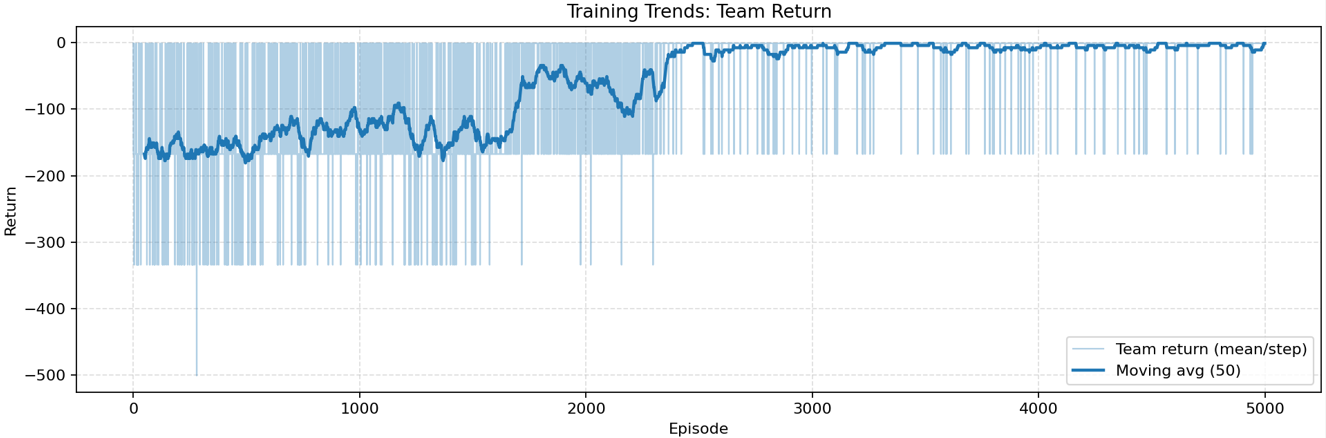
\includegraphics[width=0.75\linewidth]{VDNHist.png}
    \caption{Retour d'équipe global}
\end{figure}

\begin{figure}
    \centering
    
\includegraphics[width=0.75\linewidth]{QMIX/training_agent_rewards.png}
    \caption{Récompenses par agent}
\end{figure}
\end{frame}

\begin{frame}{4. MADDPG – Multi-Agent Actor-Critic}
\begin{center}
    \Large\textbf{MADDPG = DDPG multi-agent + CTDE}
\end{center}

Architecture :
\begin{itemize}
    \item \textbf{Actor} décentralisé : $a_i = \mu_i(o_i; \theta_i)$
    \item \textbf{Critic} centralisé : $Q_i(\mathbf{o}, \mathbf{a}; \phi_i)$
\end{itemize}

\end{frame}

\begin{frame}{Récompenses par agent – Run MADDPG (CTDE)}
\centering

\includegraphics[width=0.75\textwidth]{training_agent_rewards.png}

\smallskip

\begin{block}{Observations sur les récompenses individuelles}
\begin{itemize}
    \item Trois agents avec politiques différentes
    \item Phase initiale : progression rapide vers −100 / −50 (beaucoup plus stable que les runs indépendants)
    \item Plateau autour de −20 / 0 après ~1500–2000 épisodes
    \item Quelques oscillations locales tardives, mais amplitude faible
    \item Courbes MA(50) très proches et alignées → coordination implicite efficace
\end{itemize}
\end{block}

\end{frame}

\begin{frame}{Retour d'équipe et bilan final – MADDPG}
\centering

\includegraphics[width=0.75\textwidth]{MADDPGHis.png}

\vspace{0.4em}

\begin{block}{Analyse du Team Return (moyenne par step)}
\begin{itemize}
    \item Départ autour de \− 40
    \item Amélioration régulière et rapide → plateau stable autour de −5 / −10 après ~1500 épisodes
    \item Oscillations très faibles en phase tardive
    \item Performance finale nettement supérieure aux runs indépendants
\end{itemize}
\end{block}

\end{frame}

\begin{frame}{Résumé global de l'entraînement MADDPG}
\frametitle{Résumé global – 5000 épisodes}

\begin{block}{Informations clés}
\begin{itemize}
    \item Épisodes totaux : \textbf{5000}
    \item Durée totale : \alert{1h 53min 43s} ($\approx$ 1h54)
    \item Taux de succès environnemental final : \alert{\textbf{79.3 \%}}
    \item Épisodes échoués : 1036 / 5000
    \item Epsilon final : \textbf{0.050} (phase d'exploitation quasi-totale)
\end{itemize}
\end{block}

\smallskip

\begin{alertblock}{Interprétation}
79.3 \% de succès est un très bon résultat pour un problème multi-agent d'allocation distribuée \\
(ex. inférence DNN collaborative sur edge devices hétérogènes)
\end{alertblock}
\end{frame}

% ----------------------------------------------------
\begin{frame}{Évolution des métriques – Derniers épisodes}
\frametitle{Métriques clés des derniers épisodes}

\begin{figure}
    \centering
    \includegraphics[width=0.9\linewidth]{TimeMADDPG.png}
\end{figure}

\begin{block}{Observations principales}
\begin{itemize}
    \item Amélioration forte : de -100/-200 au milieu → \alert{-5/-10} en fin de run
    \item Récompenses individuelles très alignées → bonne coordination implicite
    \item Taux de succès individuel final : 86--92 \% → excellente exploitation
    \item Loss critique stable ($\sim$1134--1135) → apprentissage sain, pas de divergence
\end{itemize}
\end{block}
\end{frame}

% ----------------------------------------------------
\begin{frame}{Synthèse et avantages démontrés}
\frametitle{Conclusion – Performances MADDPG}

\begin{columns}[T]
\column{0.55\textwidth}
\begin{alertblock}{Points forts observés}
\begin{itemize}
    \item Convergence rapide et stable (plateau après $\sim$1500--2000 épisodes)
    \item Récompense d'équipe finale : \alert{$-5$ à $-10$} (très bon niveau)
    \item Taux de succès global : \alert{\textbf{79.3 \%}}
    \item Coordination implicite efficace malgré agents hétérogènes
    \item Stabilité tardive : pas de chute catastrophique
\end{itemize}
\end{alertblock}

\column{0.45\textwidth}
\begin{block}{Pourquoi MADDPG réussit ici ?}
\begin{itemize}
    \item Critic centralisé → réduit fortement la non-stationnarité
    \item Observation globale pendant l'entraînement → coordination apprise
    \item Meilleure robustesse que l'apprentissage indépendant
\end{itemize}
\end{block}
\end{columns}

\smallskip\centering
\Large\textbf{MADDPG confirme son avantage pour ce problème multi-agent distribué}
\end{frame}


\end{document}